\documentclass[]{article}
\usepackage{lmodern}
\usepackage{amssymb,amsmath}
\usepackage{ifxetex,ifluatex}
\usepackage{fixltx2e} % provides \textsubscript
\ifnum 0\ifxetex 1\fi\ifluatex 1\fi=0 % if pdftex
  \usepackage[T1]{fontenc}
  \usepackage[utf8]{inputenc}
\else % if luatex or xelatex
  \ifxetex
    \usepackage{mathspec}
  \else
    \usepackage{fontspec}
  \fi
  \defaultfontfeatures{Ligatures=TeX,Scale=MatchLowercase}
\fi
% use upquote if available, for straight quotes in verbatim environments
\IfFileExists{upquote.sty}{\usepackage{upquote}}{}
% use microtype if available
\IfFileExists{microtype.sty}{%
\usepackage{microtype}
\UseMicrotypeSet[protrusion]{basicmath} % disable protrusion for tt fonts
}{}
\usepackage[margin=1in]{geometry}
\usepackage{hyperref}
\hypersetup{unicode=true,
            pdftitle={Exploring Revision 5a MCMC and vb},
            pdfborder={0 0 0},
            breaklinks=true}
\urlstyle{same}  % don't use monospace font for urls
\usepackage{color}
\usepackage{fancyvrb}
\newcommand{\VerbBar}{|}
\newcommand{\VERB}{\Verb[commandchars=\\\{\}]}
\DefineVerbatimEnvironment{Highlighting}{Verbatim}{commandchars=\\\{\}}
% Add ',fontsize=\small' for more characters per line
\usepackage{framed}
\definecolor{shadecolor}{RGB}{248,248,248}
\newenvironment{Shaded}{\begin{snugshade}}{\end{snugshade}}
\newcommand{\KeywordTok}[1]{\textcolor[rgb]{0.13,0.29,0.53}{\textbf{{#1}}}}
\newcommand{\DataTypeTok}[1]{\textcolor[rgb]{0.13,0.29,0.53}{{#1}}}
\newcommand{\DecValTok}[1]{\textcolor[rgb]{0.00,0.00,0.81}{{#1}}}
\newcommand{\BaseNTok}[1]{\textcolor[rgb]{0.00,0.00,0.81}{{#1}}}
\newcommand{\FloatTok}[1]{\textcolor[rgb]{0.00,0.00,0.81}{{#1}}}
\newcommand{\ConstantTok}[1]{\textcolor[rgb]{0.00,0.00,0.00}{{#1}}}
\newcommand{\CharTok}[1]{\textcolor[rgb]{0.31,0.60,0.02}{{#1}}}
\newcommand{\SpecialCharTok}[1]{\textcolor[rgb]{0.00,0.00,0.00}{{#1}}}
\newcommand{\StringTok}[1]{\textcolor[rgb]{0.31,0.60,0.02}{{#1}}}
\newcommand{\VerbatimStringTok}[1]{\textcolor[rgb]{0.31,0.60,0.02}{{#1}}}
\newcommand{\SpecialStringTok}[1]{\textcolor[rgb]{0.31,0.60,0.02}{{#1}}}
\newcommand{\ImportTok}[1]{{#1}}
\newcommand{\CommentTok}[1]{\textcolor[rgb]{0.56,0.35,0.01}{\textit{{#1}}}}
\newcommand{\DocumentationTok}[1]{\textcolor[rgb]{0.56,0.35,0.01}{\textbf{\textit{{#1}}}}}
\newcommand{\AnnotationTok}[1]{\textcolor[rgb]{0.56,0.35,0.01}{\textbf{\textit{{#1}}}}}
\newcommand{\CommentVarTok}[1]{\textcolor[rgb]{0.56,0.35,0.01}{\textbf{\textit{{#1}}}}}
\newcommand{\OtherTok}[1]{\textcolor[rgb]{0.56,0.35,0.01}{{#1}}}
\newcommand{\FunctionTok}[1]{\textcolor[rgb]{0.00,0.00,0.00}{{#1}}}
\newcommand{\VariableTok}[1]{\textcolor[rgb]{0.00,0.00,0.00}{{#1}}}
\newcommand{\ControlFlowTok}[1]{\textcolor[rgb]{0.13,0.29,0.53}{\textbf{{#1}}}}
\newcommand{\OperatorTok}[1]{\textcolor[rgb]{0.81,0.36,0.00}{\textbf{{#1}}}}
\newcommand{\BuiltInTok}[1]{{#1}}
\newcommand{\ExtensionTok}[1]{{#1}}
\newcommand{\PreprocessorTok}[1]{\textcolor[rgb]{0.56,0.35,0.01}{\textit{{#1}}}}
\newcommand{\AttributeTok}[1]{\textcolor[rgb]{0.77,0.63,0.00}{{#1}}}
\newcommand{\RegionMarkerTok}[1]{{#1}}
\newcommand{\InformationTok}[1]{\textcolor[rgb]{0.56,0.35,0.01}{\textbf{\textit{{#1}}}}}
\newcommand{\WarningTok}[1]{\textcolor[rgb]{0.56,0.35,0.01}{\textbf{\textit{{#1}}}}}
\newcommand{\AlertTok}[1]{\textcolor[rgb]{0.94,0.16,0.16}{{#1}}}
\newcommand{\ErrorTok}[1]{\textcolor[rgb]{0.64,0.00,0.00}{\textbf{{#1}}}}
\newcommand{\NormalTok}[1]{{#1}}
\usepackage{graphicx,grffile}
\makeatletter
\def\maxwidth{\ifdim\Gin@nat@width>\linewidth\linewidth\else\Gin@nat@width\fi}
\def\maxheight{\ifdim\Gin@nat@height>\textheight\textheight\else\Gin@nat@height\fi}
\makeatother
% Scale images if necessary, so that they will not overflow the page
% margins by default, and it is still possible to overwrite the defaults
% using explicit options in \includegraphics[width, height, ...]{}
\setkeys{Gin}{width=\maxwidth,height=\maxheight,keepaspectratio}
\IfFileExists{parskip.sty}{%
\usepackage{parskip}
}{% else
\setlength{\parindent}{0pt}
\setlength{\parskip}{6pt plus 2pt minus 1pt}
}
\setlength{\emergencystretch}{3em}  % prevent overfull lines
\providecommand{\tightlist}{%
  \setlength{\itemsep}{0pt}\setlength{\parskip}{0pt}}
\setcounter{secnumdepth}{0}
% Redefines (sub)paragraphs to behave more like sections
\ifx\paragraph\undefined\else
\let\oldparagraph\paragraph
\renewcommand{\paragraph}[1]{\oldparagraph{#1}\mbox{}}
\fi
\ifx\subparagraph\undefined\else
\let\oldsubparagraph\subparagraph
\renewcommand{\subparagraph}[1]{\oldsubparagraph{#1}\mbox{}}
\fi

%%% Use protect on footnotes to avoid problems with footnotes in titles
\let\rmarkdownfootnote\footnote%
\def\footnote{\protect\rmarkdownfootnote}

%%% Change title format to be more compact
\usepackage{titling}

% Create subtitle command for use in maketitle
\newcommand{\subtitle}[1]{
  \posttitle{
    \begin{center}\large#1\end{center}
    }
}

\setlength{\droptitle}{-2em}
  \title{Exploring Revision 5a MCMC and vb}
  \pretitle{\vspace{\droptitle}\centering\huge}
  \posttitle{\par}
  \author{}
  \preauthor{}\postauthor{}
  \date{}
  \predate{}\postdate{}


\begin{document}
\maketitle

Revision 5a has the following features:

\begin{itemize}
\tightlist
\item
  includes one group of subjects
\item
  Has a level for multiple runs as random effects
\item
  Runs can be either reward, punishment, or unspecified. Each subject
  has an individual parameter specifying difference between reward and
  punishment runs, and these are drawn from a group-level distribution
  of runs.
\end{itemize}

The variational bayes estimates for Revision 5 looked good. So I ran
Revision 5 on MCMC:

\begin{itemize}
\tightlist
\item
  on each of the three groups
\item
  Using both variational bayes and MCMC
\item
  three times so that we could look at consistency across different
  runs.
\end{itemize}

\subsection{Variational Bayes: posterior
comparison}\label{variational-bayes-posterior-comparison}

Though we have already done a variational Bayes estimate (see
rev5\_exploration-vb.Rmd), here, these are presented side-by-side with
MCMC analyses for comparison.

\begin{Shaded}
\begin{Highlighting}[]
\KeywordTok{source}\NormalTok{(}\StringTok{"du_model_rev5a-mcmc1timerun.R"}\NormalTok{)}
\end{Highlighting}
\end{Shaded}

\begin{verbatim}
## [1] "initializing..."
\end{verbatim}

\begin{verbatim}
## Loading required package: hBayesDM
\end{verbatim}

\begin{verbatim}
## Loading required package: Rcpp
\end{verbatim}

\begin{verbatim}
## 
## 
## This is hBayesDM version 0.5.1
\end{verbatim}

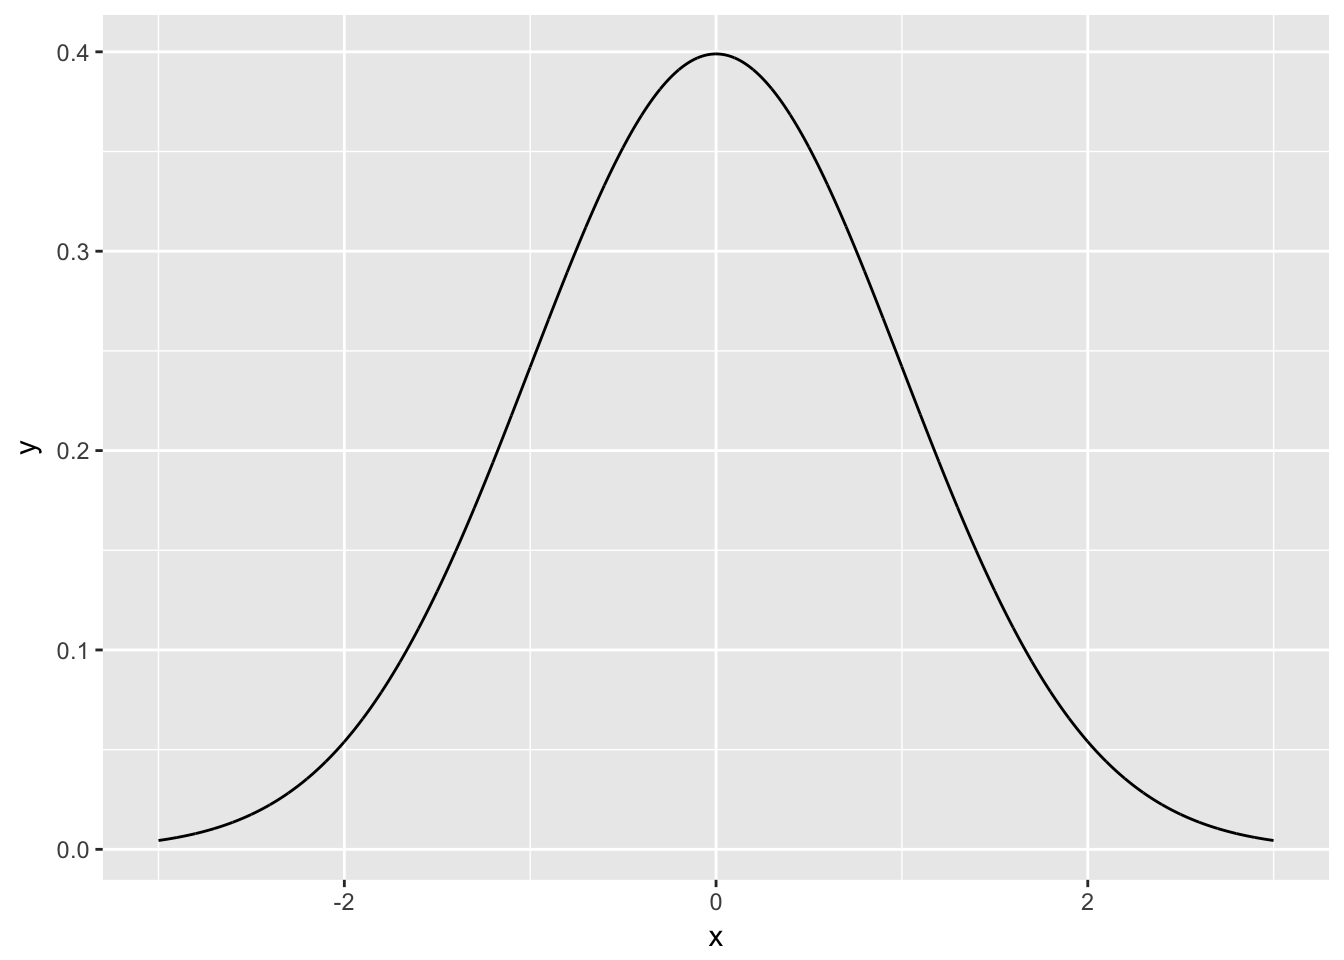
\includegraphics{rev5_exploration-2_files/figure-latex/unnamed-chunk-2-1.pdf}
\includegraphics{rev5_exploration-2_files/figure-latex/unnamed-chunk-2-2.pdf}
\includegraphics{rev5_exploration-2_files/figure-latex/unnamed-chunk-2-3.pdf}

These all look plausible. I think for the first time, I've got a model
that estimates repeated runs and reward and punishment within the same
model, and yields separate estimates for reward and punishment by using
a parameter that separates the two.

While they all look \emph{plausible}, estimates vary widely, indicating
that we need to look at MCMC in order to calculate the outcomes for
these values. Fortunately, this current model isn't unwieldy and I
should be able to run through MCMC analyses in a tractable period of
time.

\subsection{Differences}\label{differences}

I want to take a look at differences:

\begin{itemize}
\tightlist
\item
  between reward and punishment runs
\item
  between Group 2 and Group 3
\item
  An interaction of those differences.
\end{itemize}

\begin{verbatim}
## Warning in `[.data.table`(model.summary.all.rewpun, ,
## `:=`(rew_minus_pun_mu, : Invalid .internal.selfref detected and fixed
## by taking a (shallow) copy of the data.table so that := can add this new
## column by reference. At an earlier point, this data.table has been copied
## by R (or been created manually using structure() or similar). Avoid key<-,
## names<- and attr<- which in R currently (and oddly) may copy the whole
## data.table. Use set* syntax instead to avoid copying: ?set, ?setnames and ?
## setattr. Also, in R<=v3.0.2, list(DT1,DT2) copied the entire DT1 and DT2
## (R's list() used to copy named objects); please upgrade to R>v3.0.2 if that
## is biting. If this message doesn't help, please report to datatable-help so
## the root cause can be fixed.
\end{verbatim}

\begin{verbatim}
##          iter Run Parameter TestId Group           ModelName
##      1:     1 All     alpha      1     1 double_update_rev5a
##      2:     1 All     alpha      2     2 double_update_rev5a
##      3:     1 All     alpha      3     3 double_update_rev5a
##      4:     1 All     alpha      4     1 double_update_rev5a
##      5:     1 All     alpha      5     2 double_update_rev5a
##     ---                                                     
## 323924: 48000 All     alpha      2     2 double_update_rev5a
## 323925: 48000 All     alpha      3     3 double_update_rev5a
## 323926: 48000 All      beta      1     1 double_update_rev5a
## 323927: 48000 All      beta      2     2 double_update_rev5a
## 323928: 48000 All      beta      3     3 double_update_rev5a
##         AnalysisRepetition EstimationMethod    rew_mu    pun_mu
##      1:                  1             MCMC 0.3253670 0.4013265
##      2:                  1             MCMC 0.3158299 0.3744320
##      3:                  1             MCMC 0.2462382 0.2674455
##      4:                  1 variationalbayes 0.3229920 0.3862500
##      5:                  1 variationalbayes 0.3183860 0.2937640
##     ---                                                        
## 323924:                  1             MCMC 0.3103962 0.3346431
## 323925:                  1             MCMC 0.1837489 0.1793888
## 323926:                  1             MCMC 0.6338423 0.5454490
## 323927:                  1             MCMC 0.7020964 0.6493959
## 323928:                  1             MCMC 0.6900773 0.7203194
##         rew_minus_pun_mu
##      1:      -0.07595953
##      2:      -0.05860209
##      3:      -0.02120736
##      4:      -0.06325800
##      5:       0.02462200
##     ---                 
## 323924:      -0.02424691
## 323925:       0.00436020
## 323926:       0.08839326
## 323927:       0.05270057
## 323928:      -0.03024212
\end{verbatim}

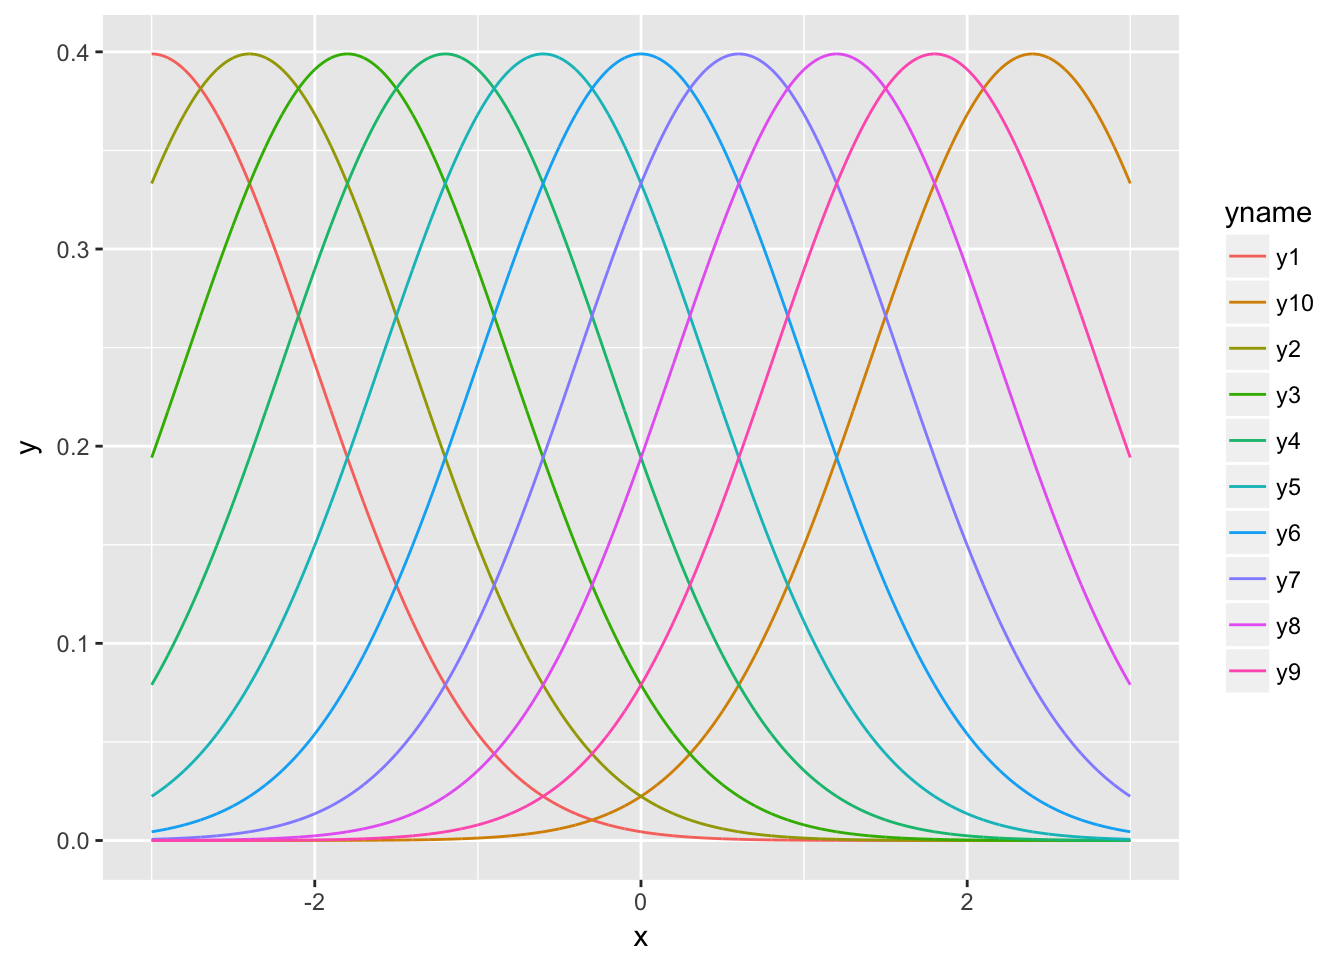
\includegraphics{rev5_exploration-2_files/figure-latex/unnamed-chunk-3-1.pdf}
\includegraphics{rev5_exploration-2_files/figure-latex/unnamed-chunk-3-2.pdf}
\includegraphics{rev5_exploration-2_files/figure-latex/unnamed-chunk-3-3.pdf}

\begin{Shaded}
\begin{Highlighting}[]
\CommentTok{# group 2 compared to group 3.}
\NormalTok{model.summary.all.notestid <-}\StringTok{ }\NormalTok{model.summary.all[, }\StringTok{`}\DataTypeTok{:=}\StringTok{`}\NormalTok{(TestId, }\OtherTok{NULL}\NormalTok{)]}

\NormalTok{model.summary.all.groupcompare <-}\StringTok{ }\NormalTok{tidyr::}\KeywordTok{spread}\NormalTok{(model.summary.all.notestid, }
    \NormalTok{Group, Value, }\DataTypeTok{sep =} \StringTok{""}\NormalTok{)}
\NormalTok{model.summary.all.groupcompare$Group3_minus_Group2 <-}\StringTok{ }\NormalTok{model.summary.all.groupcompare$Group3 -}\StringTok{ }
\StringTok{    }\NormalTok{model.summary.all.groupcompare$Group2}

\KeywordTok{ggplot}\NormalTok{(model.summary.all.groupcompare[EstimationMethod ==}\StringTok{ "variationalbayes"}\NormalTok{], }
    \KeywordTok{aes}\NormalTok{(}\DataTypeTok{x =} \NormalTok{Group3_minus_Group2, }\DataTypeTok{fill =} \KeywordTok{factor}\NormalTok{(AnalysisRepetition), }\DataTypeTok{color =} \KeywordTok{factor}\NormalTok{(AnalysisRepetition))) +}\StringTok{ }
\StringTok{    }\KeywordTok{geom_freqpoly}\NormalTok{(}\DataTypeTok{alpha =} \FloatTok{0.9}\NormalTok{, }\DataTypeTok{binwidth =} \FloatTok{0.001}\NormalTok{) +}\StringTok{ }\KeywordTok{geom_hdi}\NormalTok{(}\DataTypeTok{size =} \DecValTok{2}\NormalTok{, }\DataTypeTok{lineend =} \StringTok{"round"}\NormalTok{, }
    \DataTypeTok{alpha =} \FloatTok{0.5}\NormalTok{, }\DataTypeTok{credible_mass =} \FloatTok{0.95}\NormalTok{) +}\StringTok{ }\KeywordTok{facet_grid}\NormalTok{(Statistic ~}\StringTok{ }\NormalTok{Parameter, }\DataTypeTok{scales =} \StringTok{"free"}\NormalTok{) +}\StringTok{ }
\StringTok{    }\KeywordTok{labs}\NormalTok{(}\DataTypeTok{title =} \KeywordTok{paste0}\NormalTok{(}\StringTok{"mu statistic (all rounds), Group 3 Minus Group 2"}\NormalTok{))}
\end{Highlighting}
\end{Shaded}

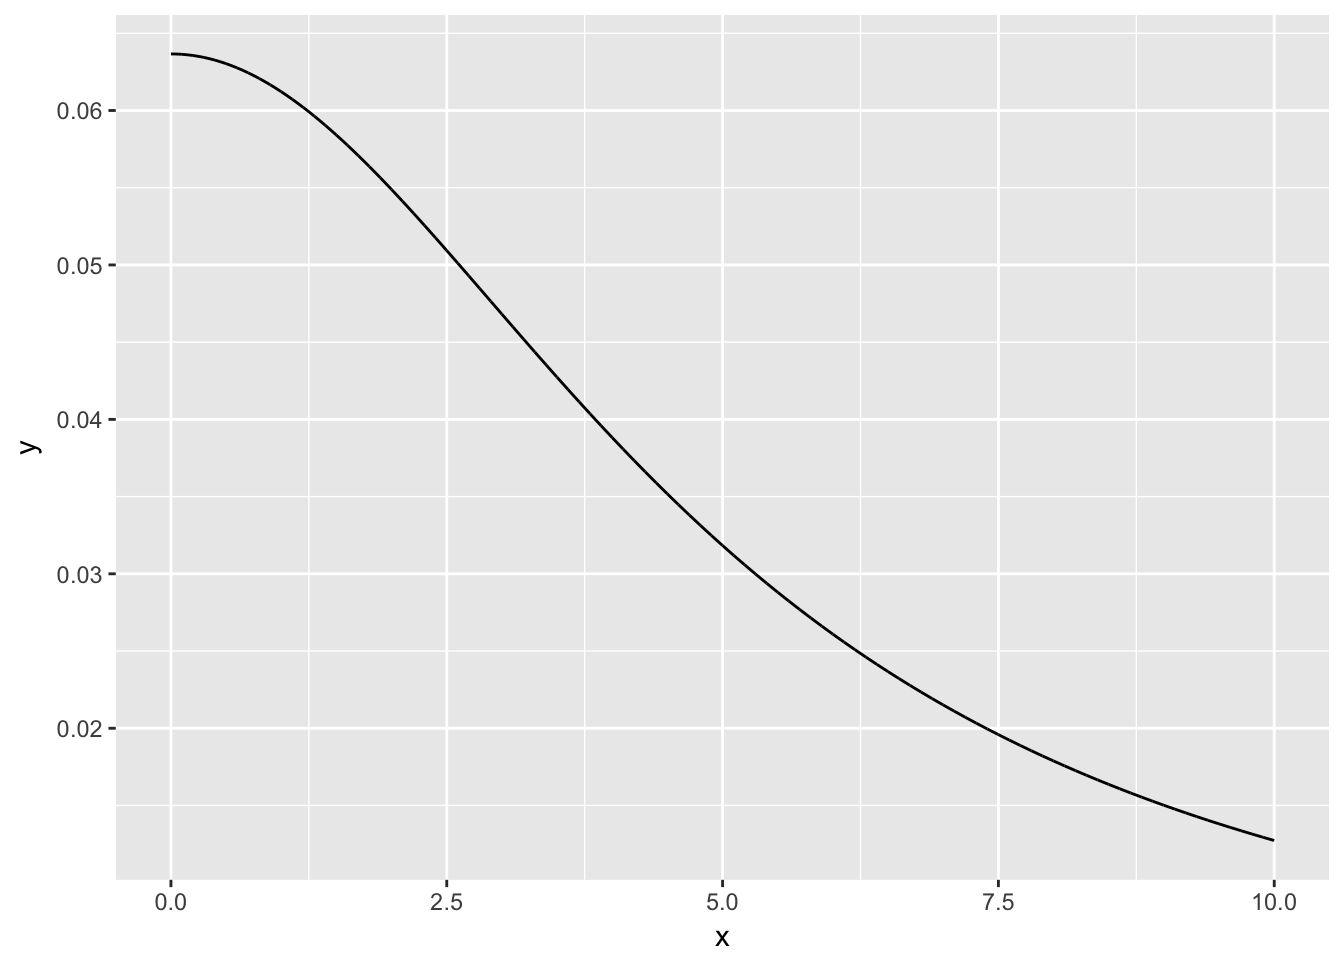
\includegraphics{rev5_exploration-2_files/figure-latex/unnamed-chunk-4-1.pdf}

These all look like plausible estimates of group-level parameters.

\subsection{Exploring the structure of the
parameters}\label{exploring-the-structure-of-the-parameters}

Can we take a peak at how \ldots{}..

\section{MCMC results}\label{mcmc-results}

Let's take a look at the same distributions using MCMC.

\includegraphics{rev5_exploration-2_files/figure-latex/unnamed-chunk-5-1.pdf}
\includegraphics{rev5_exploration-2_files/figure-latex/unnamed-chunk-5-2.pdf}

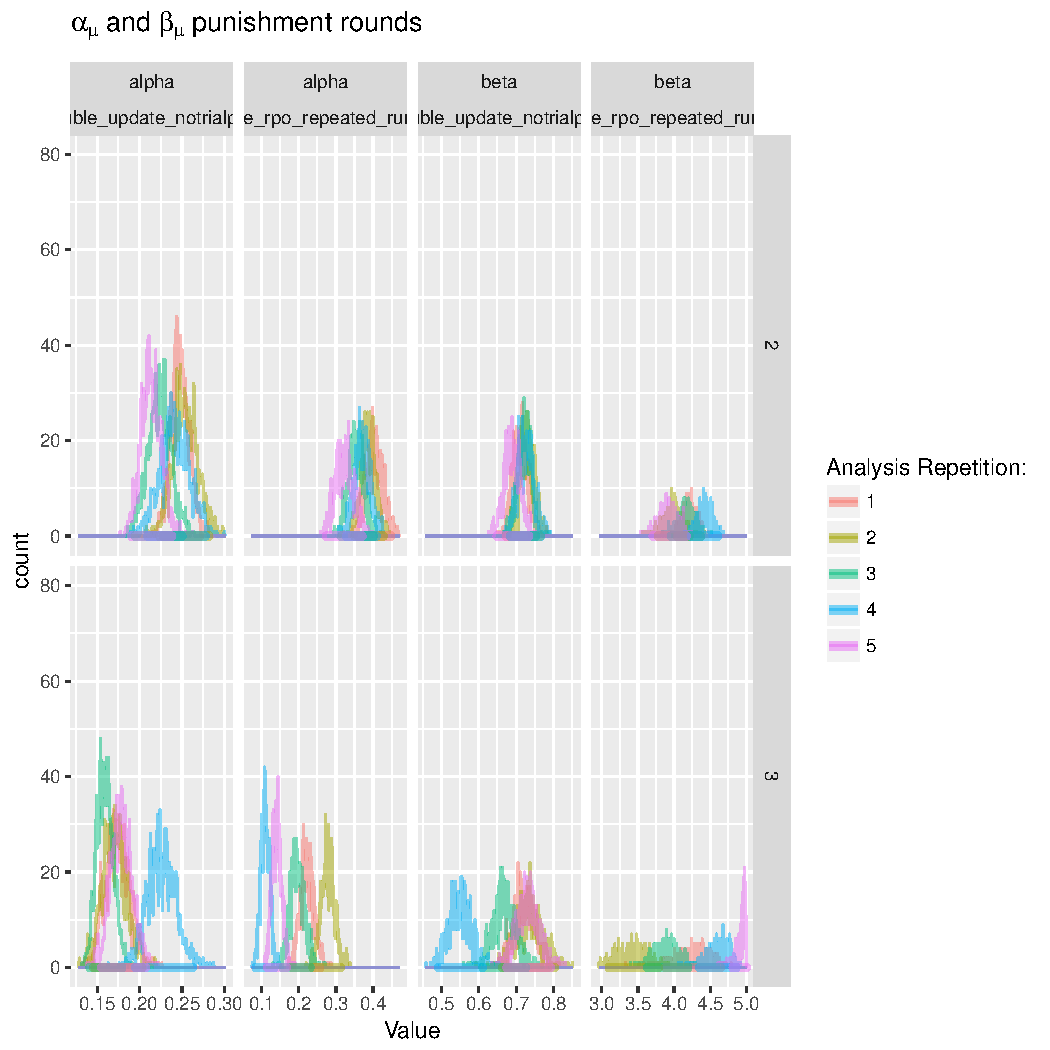
\includegraphics{rev5_exploration-2_files/figure-latex/unnamed-chunk-6-1.pdf}
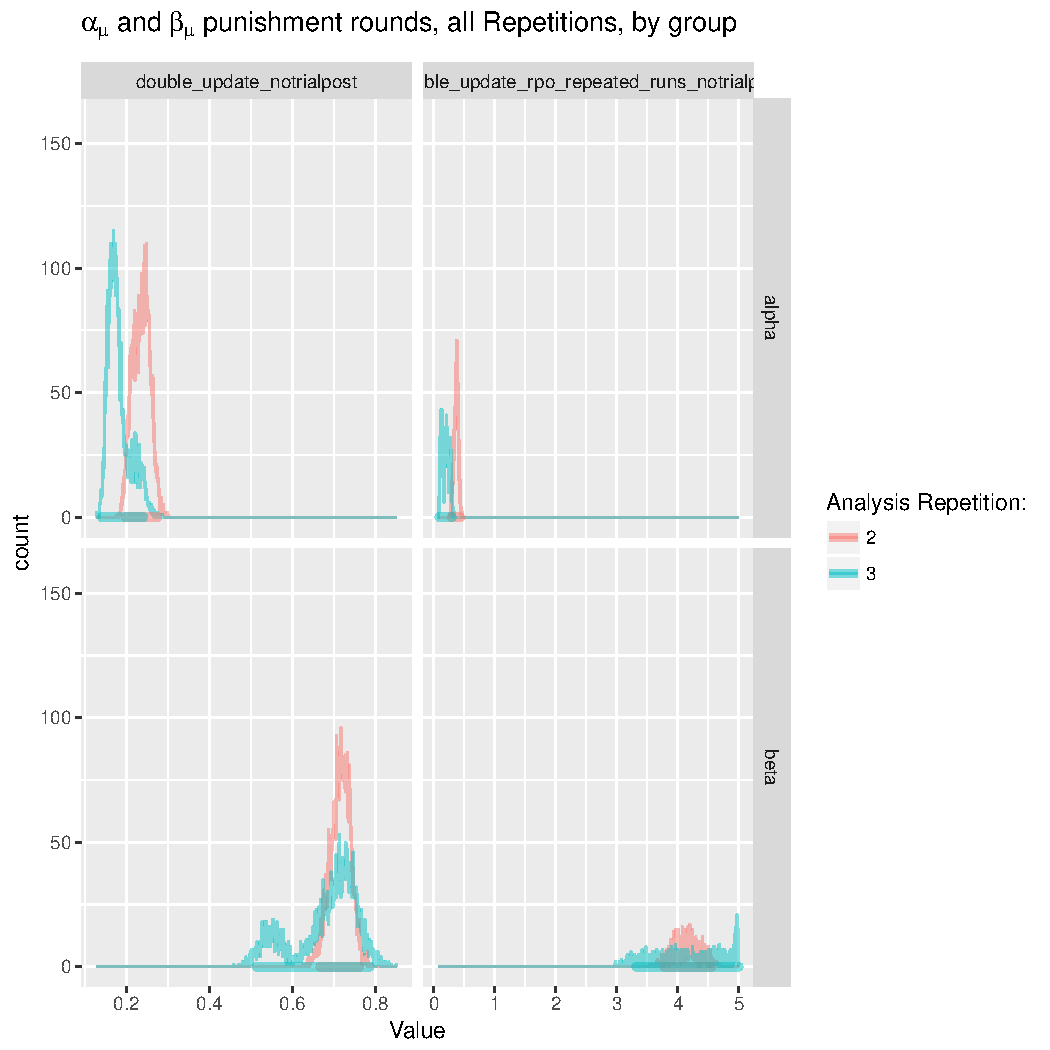
\includegraphics{rev5_exploration-2_files/figure-latex/unnamed-chunk-6-2.pdf}
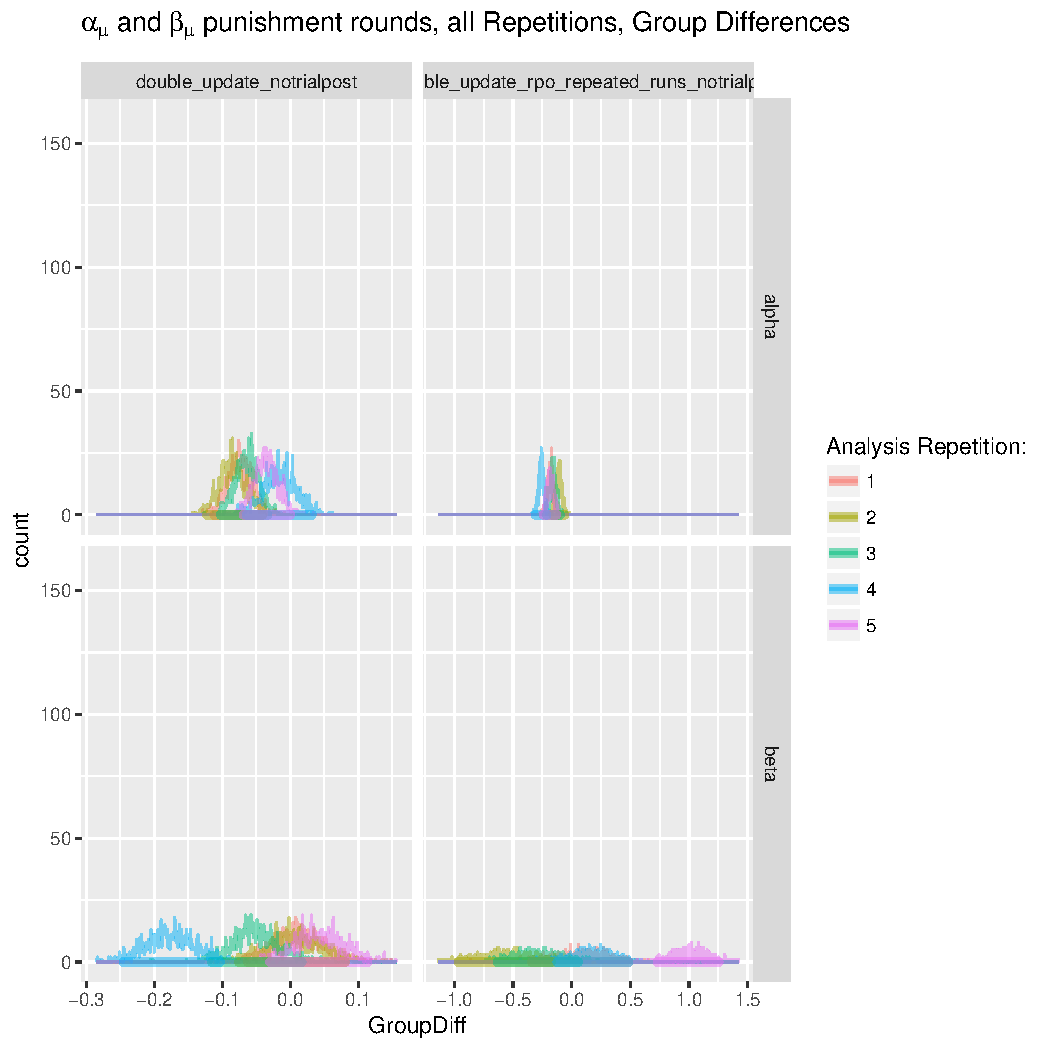
\includegraphics{rev5_exploration-2_files/figure-latex/unnamed-chunk-6-3.pdf}

Need to check the scale these reward and punishment parameters are on.
Are they transformed into the actual space there implemented within?

\begin{Shaded}
\begin{Highlighting}[]
\CommentTok{#group 2 compared to group 3.}
\NormalTok{model.summary.all.notestid<-model.summary.all[,TestId:}\ErrorTok{=}\OtherTok{NULL}\NormalTok{] }
\end{Highlighting}
\end{Shaded}

\begin{verbatim}
## Warning in `[.data.table`(model.summary.all, , `:=`(TestId, NULL)): Adding
## new column 'TestId' then assigning NULL (deleting it).
\end{verbatim}

\begin{Shaded}
\begin{Highlighting}[]
\NormalTok{model.summary.all.groupcompare<-}\StringTok{ }\NormalTok{tidyr::}\KeywordTok{spread}\NormalTok{(model.summary.all.notestid,Group,Value,}\DataTypeTok{sep=}\StringTok{""}\NormalTok{)}
\NormalTok{model.summary.all.groupcompare$Group3_minus_Group2<-}
\StringTok{  }\NormalTok{model.summary.all.groupcompare$Group3-model.summary.all.groupcompare$Group2}


\KeywordTok{ggplot}\NormalTok{(model.summary.all.groupcompare[EstimationMethod==}\StringTok{"MCMC"}\NormalTok{],}\KeywordTok{aes}\NormalTok{(}\DataTypeTok{x=}\NormalTok{Group3_minus_Group2 ,}\DataTypeTok{fill=}\KeywordTok{factor}\NormalTok{(AnalysisRepetition),}\DataTypeTok{color=}\KeywordTok{factor}\NormalTok{(AnalysisRepetition)}
                                                               \NormalTok{))+}
\StringTok{    }\KeywordTok{geom_freqpoly}\NormalTok{(}\DataTypeTok{alpha=}\FloatTok{0.9}\NormalTok{,}\DataTypeTok{binwidth=}\FloatTok{0.001}\NormalTok{)+}
\StringTok{     }\KeywordTok{geom_hdi}\NormalTok{(}\DataTypeTok{size=}\DecValTok{2}\NormalTok{, }\DataTypeTok{lineend =} \StringTok{"round"}\NormalTok{,}\DataTypeTok{alpha=}\FloatTok{0.5}\NormalTok{,}\DataTypeTok{credible_mass=}\FloatTok{0.95}\NormalTok{)+}
\StringTok{    }\KeywordTok{facet_grid}\NormalTok{(Statistic~Parameter,}\DataTypeTok{scales =} \StringTok{"free"}\NormalTok{)+}
\StringTok{    }\KeywordTok{labs}\NormalTok{(}\DataTypeTok{title=}\KeywordTok{paste0}\NormalTok{(}\StringTok{"mu statistic (all rounds), Group 3 Minus Group 2"}\NormalTok{))}
\end{Highlighting}
\end{Shaded}

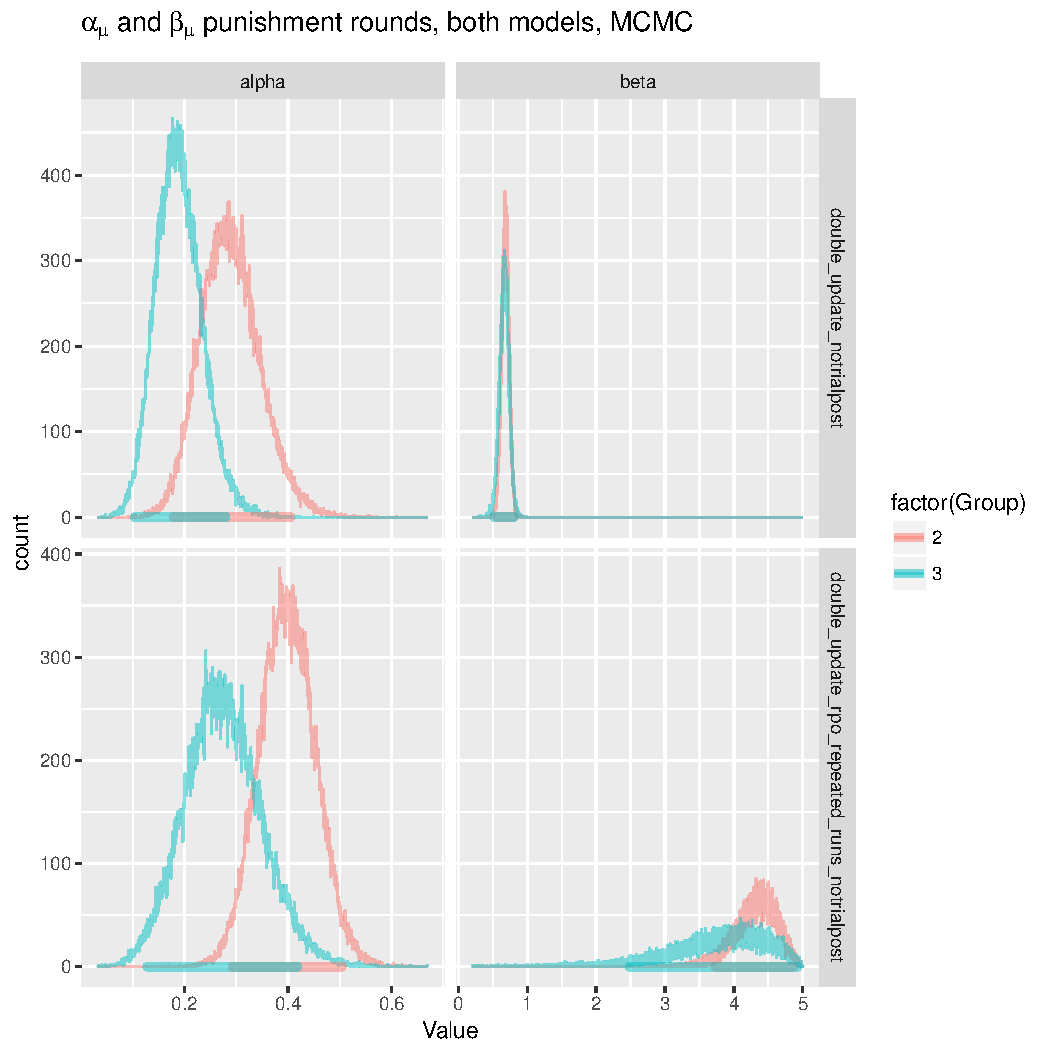
\includegraphics{rev5_exploration-2_files/figure-latex/unnamed-chunk-7-1.pdf}

\begin{Shaded}
\begin{Highlighting}[]
\KeywordTok{head}\NormalTok{(model.summary.all.groupcompare)}
\end{Highlighting}
\end{Shaded}

\begin{verbatim}
##    iter Run Statistic Parameter           ModelName AnalysisRepetition
## 1:    1 All        mu     alpha double_update_rev5a                  1
## 2:    1 All        mu     alpha double_update_rev5a                  1
## 3:    1 All        mu     alpha double_update_rev5a                  2
## 4:    1 All        mu     alpha double_update_rev5a                  3
## 5:    1 All        mu     alpha double_update_rev5a                  4
## 6:    1 All        mu     alpha double_update_rev5a                  5
##    EstimationMethod     Group1    Group2    Group3 Group3_minus_Group2
## 1:             MCMC 0.36266527 0.3446611 0.2567271         -0.08793403
## 2: variationalbayes 0.35411300 0.3059640 0.2504850         -0.05547900
## 3: variationalbayes 0.00942966 0.2985100 0.0860701         -0.21243990
## 4: variationalbayes 0.02321940 0.0274609 0.4028540          0.37539310
## 5: variationalbayes 0.28699100 0.3255150 0.2894890         -0.03602600
## 6: variationalbayes 0.29553300 0.4532400 0.1735660         -0.27967400
\end{verbatim}

\begin{Shaded}
\begin{Highlighting}[]
\NormalTok{model.summary.all.g3g2compare.bypar<-}\StringTok{ }
\StringTok{  }\NormalTok{tidyr::}\KeywordTok{spread}\NormalTok{(}
    \NormalTok{model.summary.all.groupcompare[,.(iter,Run,Statistic,Parameter,ModelName,AnalysisRepetition,}
                                   \NormalTok{EstimationMethod,Group3_minus_Group2)],}
    \NormalTok{Parameter,}
    \NormalTok{Group3_minus_Group2)}

\KeywordTok{ggplot}\NormalTok{(model.summary.all.g3g2compare.bypar[}
  \NormalTok{EstimationMethod==}\StringTok{"MCMC"} \NormalTok{&}\StringTok{ }
\StringTok{  }\NormalTok{Statistic %in%}\StringTok{ }\KeywordTok{c}\NormalTok{(}\StringTok{"mu"}\NormalTok{,}\StringTok{"rew_mu"}\NormalTok{,}\StringTok{"pun_mu"}\NormalTok{)}
                                              \NormalTok{],}\KeywordTok{aes}\NormalTok{(}\DataTypeTok{x=}\NormalTok{alpha,}\DataTypeTok{y=}\NormalTok{beta }
                                                    \CommentTok{#,fill=factor(Statistic),color=factor(Statistic)}
                                                    \NormalTok{))+}
\StringTok{    }\KeywordTok{geom_point}\NormalTok{(}\DataTypeTok{alpha=}\FloatTok{0.1}\NormalTok{)+}
\StringTok{    }\KeywordTok{facet_grid}\NormalTok{(~Statistic,}\DataTypeTok{scales =} \StringTok{"free"}\NormalTok{)+}
\StringTok{    }\KeywordTok{labs}\NormalTok{(}\DataTypeTok{title=}\KeywordTok{paste0}\NormalTok{(}\StringTok{"mu statistic (all rounds), Group 3 Minus Group 2"}\NormalTok{))}
\end{Highlighting}
\end{Shaded}

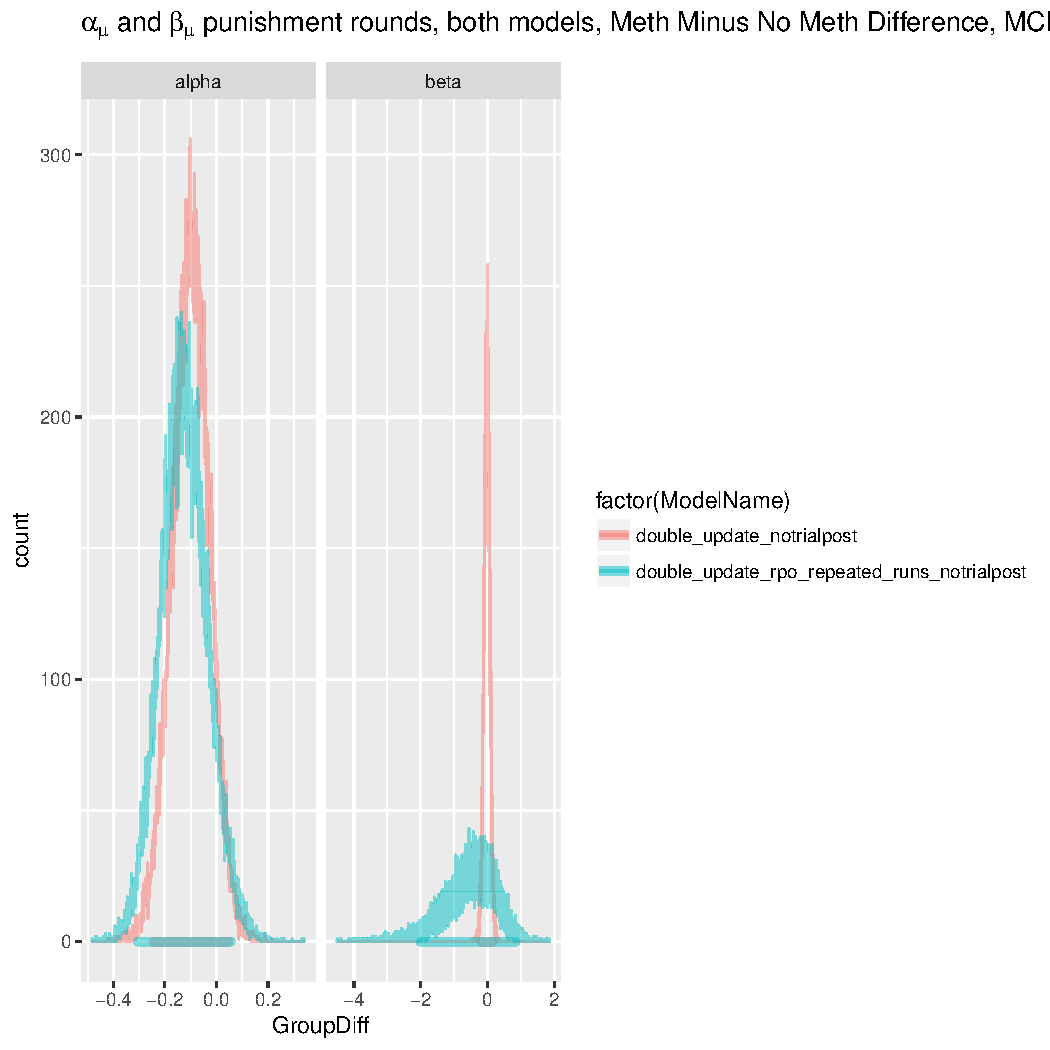
\includegraphics{rev5_exploration-2_files/figure-latex/unnamed-chunk-7-2.pdf}

\begin{Shaded}
\begin{Highlighting}[]
\CommentTok{# group 1 compared to group 2}
\NormalTok{model.summary.all.groupcompare$Group2_minus_Group1 <-}\StringTok{ }\NormalTok{model.summary.all.groupcompare$Group2 -}\StringTok{ }
\StringTok{    }\NormalTok{model.summary.all.groupcompare$Group1}

\KeywordTok{ggplot}\NormalTok{(model.summary.all.groupcompare[EstimationMethod ==}\StringTok{ "MCMC"}\NormalTok{], }\KeywordTok{aes}\NormalTok{(}\DataTypeTok{x =} \NormalTok{Group2_minus_Group1, }
    \DataTypeTok{fill =} \KeywordTok{factor}\NormalTok{(AnalysisRepetition), }\DataTypeTok{color =} \KeywordTok{factor}\NormalTok{(AnalysisRepetition))) +}\StringTok{ }
\StringTok{    }\KeywordTok{geom_freqpoly}\NormalTok{(}\DataTypeTok{alpha =} \FloatTok{0.9}\NormalTok{, }\DataTypeTok{binwidth =} \FloatTok{0.001}\NormalTok{) +}\StringTok{ }\KeywordTok{geom_hdi}\NormalTok{(}\DataTypeTok{size =} \DecValTok{2}\NormalTok{, }\DataTypeTok{lineend =} \StringTok{"round"}\NormalTok{, }
    \DataTypeTok{alpha =} \FloatTok{0.5}\NormalTok{, }\DataTypeTok{credible_mass =} \FloatTok{0.95}\NormalTok{) +}\StringTok{ }\KeywordTok{facet_grid}\NormalTok{(Statistic ~}\StringTok{ }\NormalTok{Parameter, }\DataTypeTok{scales =} \StringTok{"free"}\NormalTok{) +}\StringTok{ }
\StringTok{    }\KeywordTok{labs}\NormalTok{(}\DataTypeTok{title =} \KeywordTok{paste0}\NormalTok{(}\StringTok{"mu statistic (all rounds), Group 2 Minus Group 1"}\NormalTok{))}
\end{Highlighting}
\end{Shaded}

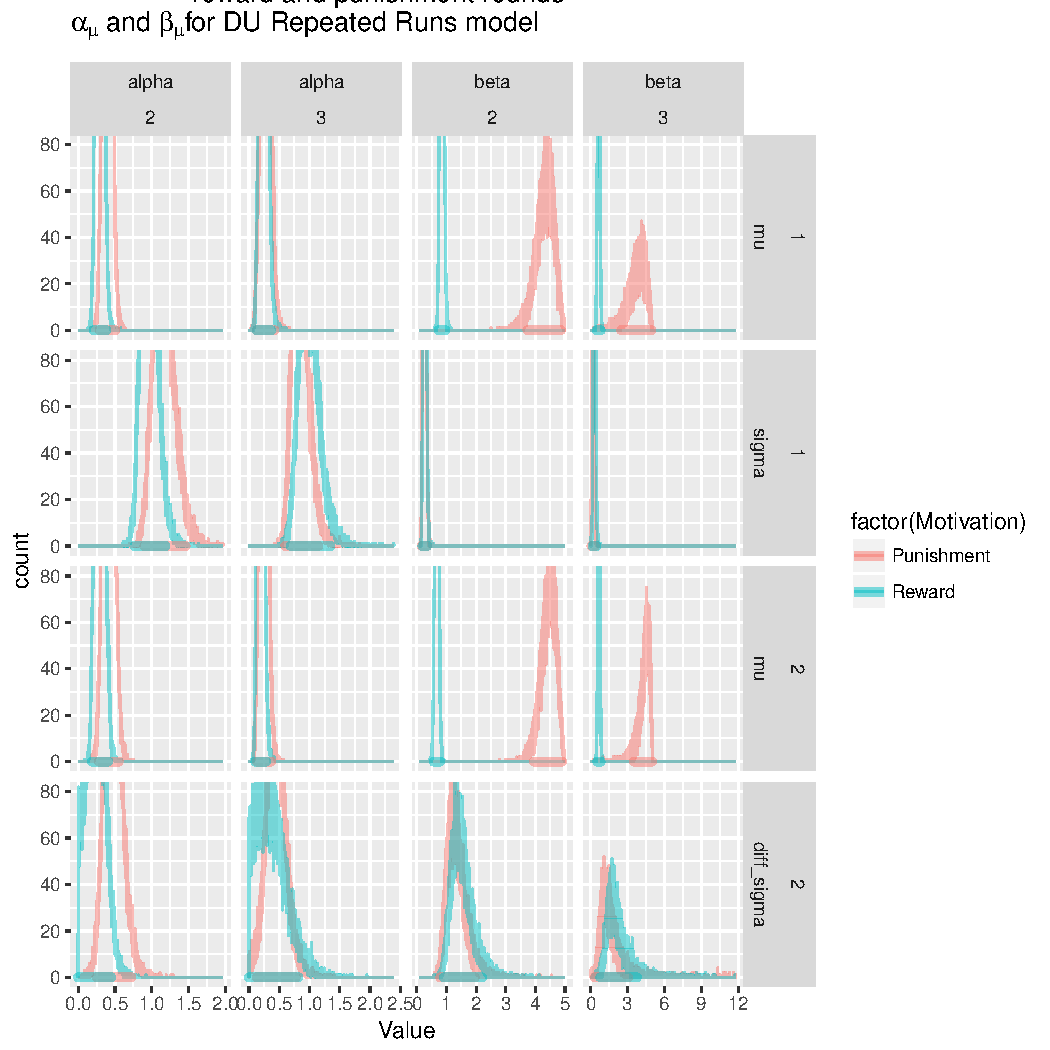
\includegraphics{rev5_exploration-2_files/figure-latex/unnamed-chunk-8-1.pdf}

\begin{Shaded}
\begin{Highlighting}[]
\NormalTok{model.summary.all.g2g1compare.bypar <-}\StringTok{ }\NormalTok{tidyr::}\KeywordTok{spread}\NormalTok{(model.summary.all.groupcompare[, }
    \NormalTok{.(iter, Run, Statistic, Parameter, ModelName, AnalysisRepetition, EstimationMethod, }
        \NormalTok{Group2_minus_Group1)], Parameter, Group2_minus_Group1)}

\KeywordTok{ggplot}\NormalTok{(model.summary.all.g2g1compare.bypar[EstimationMethod ==}\StringTok{ "MCMC"} \NormalTok{&}\StringTok{ }\NormalTok{Statistic %in%}\StringTok{ }
\StringTok{    }\KeywordTok{c}\NormalTok{(}\StringTok{"mu"}\NormalTok{, }\StringTok{"rew_mu"}\NormalTok{, }\StringTok{"pun_mu"}\NormalTok{)], }\KeywordTok{aes}\NormalTok{(}\DataTypeTok{x =} \NormalTok{alpha, }\DataTypeTok{y =} \NormalTok{beta)) +}\StringTok{ }\KeywordTok{geom_point}\NormalTok{(}\DataTypeTok{alpha =} \FloatTok{0.02}\NormalTok{) +}\StringTok{ }
\StringTok{    }\KeywordTok{facet_grid}\NormalTok{(~Statistic, }\DataTypeTok{scales =} \StringTok{"free"}\NormalTok{) +}\StringTok{ }\KeywordTok{labs}\NormalTok{(}\DataTypeTok{title =} \KeywordTok{paste0}\NormalTok{(}\StringTok{"mu statistic (all rounds), Group 2 Minus Group 1"}\NormalTok{))}
\end{Highlighting}
\end{Shaded}

\includegraphics{rev5_exploration-2_files/figure-latex/unnamed-chunk-8-2.pdf}


\end{document}
